\title{System Dynamics:  Exercise 1 - Petri Dish}
\author{Ryan Spangler}
\date{\today}

\documentclass[12pt]{article}

\usepackage{graphicx}

\begin{document}
\maketitle

\section{Approach}

I set out to model the simple petri dish system with the hope that I would gain insight into the modeling process and become more comfortable with the concepts and tools associated with systems dynamics.  I was drawn to the petri dish model because of its biological orientation and its simplicity as a subject for an initial attempt at modeling population dynamics.  

The model I finally arrived at consists of two stocks, the nutrient and the population, and three flows:  the consumption of the nutrient, and the birth and death rates of the population.  In addition to this there are three main parameters, which correspond to weights or modifiers of the three basic flows:  the fractional consumption rate, the fractional birth rate and the fractional death rate.  When observing the various behaviors of the system, these are the parameters I was changing to produce different dynamics.  

Of course every model has its host of accompanying assumptions, and this one is no different.  Beyond the basic assumptions that the amount of nutrient does not grow and that the nutrient is evenly dispersed throughout the solution, one of the main assumptions I made is that the nutrient would be a continuous concentration rather than a collection of discrete units, and that the bacteria would reproduce at a rate relative to this concentration.  Meaning the bacteria could not reproduce in the absence of the nutrient, and would reproduce more slowly if less of the nutrient was present.   

\section{Process}

One of the first things I noticed was how many options I had in putting the model together!  For such a simple system, I had assumed that it would be a straightforward process of translating the ideas I had about it into a workable stock and flow model, but immediately I was faced with a wilderness of decisions about how to compose the various elements of the model.  One of the first decisions I had to make was whether to have the nutrient stock connected directly by a flow to the population, or to have the diminishing stock of the nutrient affect the population through more indirect means, like the birth rate or a variable affecting the birth rate.  This decision too maps to a conceptual distinction, whether nutrients are translated {\em directly} into population, or whether nutrients contribute to processes that lead to increases in population, but do not {\em become} that population.  Though it was more of a judgment call, I felt that there is enough of a difference between nutrients and the populations that consume them that the nutrients do not directly {\em become} the population, but rather affect the rate at which the population changes.  I started with the two stocks connected directly with a flow from nutrient to population, but I ended up decoupling them and having each affect the other through arrows to the respective rates in accordance with these reflections.  

Here is the model with the nutrient flowing directly into the population:

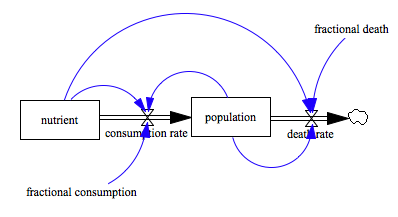
\includegraphics[scale=0.8]{initialmodel.png}

And here is the model I eventually ended up with, having the two stocks interact indirectly through arrows between the various rates:

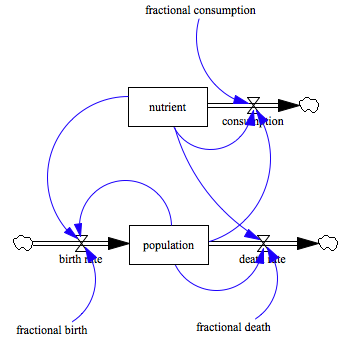
\includegraphics[scale=0.8]{finalmodel.png}

The main feedback loops I identified in the model are the reinforcing one from the population back to its birth rate, the balancing loop from population the the death rate where the higher population leads to a higher rate of death, and the balancing loop from the population to the consumption rate, where an increasing population leads to a reduction in the nutrient store, which then reduces the birth rate of the population.  Throughout all of the runs one or the other of these would dominate for awhile before another one took over, or the population died entirely.  One of the most interesting parts of the assigment was identifying which results corresponded most strongly to which loop, and observing the overlay of several loops as the system went from one phase of its dynamics to another.  

One of the things I had to work around with VensimPLE was capturing the idea that there was a fixed amount of nutrients, and that a value below zero is not meaningful.  It had a field that could be set in the nutrient stock for ``minimum value'' but when I entered zero, it would only warn me that the value had gone below minimum at a certain time step, merrily marching down further into negative territory.  I got around this finally by adding an IF THEN ELSE to only flow if the nutrient stock was above zero, but this seemed like a hack to me.  And even then, it would still stop somewhere below zero, so that I had to add a rule into the nutrient stock itself to say if the value ever got below zero, the value {\em was} zero.  Additionally, I added an IF THEN ELSE to the birth rate also to only flow if the nutrient stock was above zero.  This was dissatisfying as it seemed to be inserting the notion that the birth rate would cease if the nutrient was gone rather than having this effect emerge from the dynamics of the system, so I later replaced that scheme with having the birth rate depend directly on the amount of nutrient left.  This could be justified possibly by assuming that as the nutrient stock throughout the petri dish was deplenished (uniformly) each bacteria would have a smaller concentration in which to ingest per unit time.  

One of the main breakthroughs I made during the process was finally making the death rate inversely proportional to the amount of nutrient remaining, thereby creating a fourth reinforcing loop between the amount of nutrients and the population which consumes them.  I had assumed that having the birth rate dependent on the concentration of nutrients would be enough to limit the eventual growth of the population once the nutrients ran out, but that lead only to a balanced rise and fall, rather than the sharp dropoff I was expecting from the model.  It took increasing the death rate in the face of falling nutrients to finally show correct behavior.  

\section{Results}

With the right set of parameters and with all of the loops in the right places, this is the basic archetype of the behavior I observed:

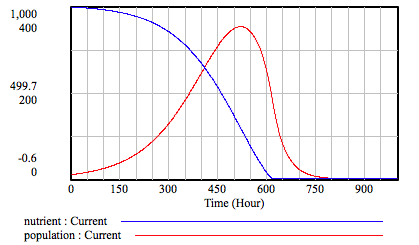
\includegraphics[scale=0.72]{archetype.png}

Notice the population begins to decline before the nutrient is fully depleted.  This is due to the influence of the nutrient store upon the birth rate, and the nutrient being absorbed at a rate corresponding to its concentration.  In the case where the population peaks and begins declining before the nutrient is gone, the death rate has exceeded the ability of the population to reproduce in the face of dwindling nutrient.  

One of the results of this system is that as I decreased the fractional consumption rate, the time scale of the nutrient stock over time did not change much, but the size of the population at its peak was raised dramatically.  I had assumed as I decreased the fractional consumption rate the nutrient would last for a longer period of time (as it wasn't being consumed as quickly), so this result surprised me.  My explanation is that since the nutrient is being depleted at a lower rate, this led to less of a dampening of the birth rate and a corresponding increase in population, leading to higher consumption overall, even though the rate of consumption was lower.  

In the above graph, the fractional consumption rate is 0.01.  Here is the same system as the archetype above with the fractional consumption rate at 0.001, and order of magnitude lower:

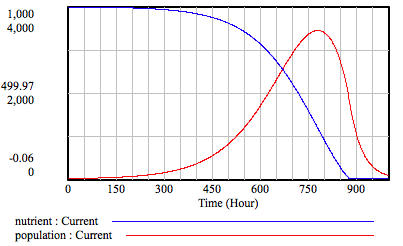
\includegraphics[scale=0.72]{lowconsumptionrate.png}

It takes a longer time to reach the peak in the graph with the lower consumption rate than the original, and the population is off to a bit of a slower start at the lower rate.  So there is a difference in the time scale of the two populations, but much less than the order of magnitude we reduced the fractional consumption rate.  However, they are dramatically different in terms of the size of the population at its peak.  In the first one, with a higher consumption rate, the population reached under 400, while in the lower one, with the consumption rate an order of magnitude lower, the population reaches a size of almost 4000, an order of magnitude higher!  Clearly the consumption rate has everything to do with the carrying capacity of the population, and not much to do with how long it takes the nutrient to be depleted and the life cycle of the population as a whole.  I found this a suprising result.  

Another interesting result is the effect of increasing the death rate.  I had assumed increasing the death rate would lead to the bacteria being alive for a shorter period of time, when in actuality an increase in the death rate would lead to the population living overall for a longer period of time, yet at a lower total size.  In the end I attribute this to the balancing loop between the size of the population and the death rate.  

In correspondence with that result, when I increased the birth rate the population peaked higher, but much quicker than at the lower rate:  


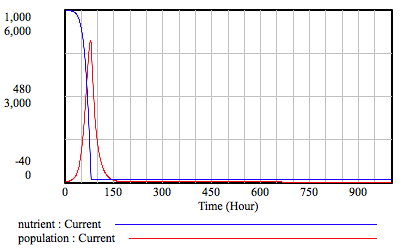
\includegraphics[scale=0.72]{highbirthrate.png}

This is in accordance with the fact that the nutrient store remained fixed, even though the population was higher.  So the higher initial population ate through its nutrients much quicker, and therefore starved much sooner.  

Overall the model reflected the RBP I was going on, so I consider it a success.  If I were to develop the model further I would have the nutrient store be a population unto itself, as suggested in the exercise description, with a birth rate and dynamics of its own.  I would be curious to see what kind of behavior I could achieve with a dual population in this way.  

\section{Equations}

Here are the resulting equations from the various stocks, flows and variables in the model:

\begin{verbatim}
  initial nutrient concentration = 1000
  initial population size = 10
  fractional consumption rate = 0.01
  fractional birth rate = 0.00001
  fractional death rate = 1.0
  consumption rate = fractional consumption rate*population
  nutrient = INTEGRAL(-consumption rate)
  birth rate = nutrient*population*fractional birth rate
  death rate = population*fractional death rate/(nutrient+40)
  population = INTEGRAL(birth rate - death rate)
\end{verbatim}



\end{document}